% Surrogate-gated loop, drawn in the visual vocabulary of the template's own
% TikZ figures (grey layer boxes, maroon flow arrows, white chips, maroon band).
\newcommand{\loopdiagram}{%
\resizebox{\linewidth}{!}{%
\begin{tikzpicture}[
  x=1cm,y=1cm,
  layer/.style = {draw=DarkGrey,line width=1.4pt,rounded corners=5pt,fill=PanelGrey},
  lbl/.style   = {font=\fontsize{28}{32}\selectfont\bfseries,text=AggieMaroon},
  sub/.style   = {font=\fontsize{22}{26}\selectfont,text=DarkGrey},
  note/.style  = {font=\fontsize{22}{26}\selectfont,text=DarkGrey},
  notem/.style = {font=\fontsize{23}{27}\selectfont\bfseries,text=AggieMaroon},
  chip/.style  = {draw=DarkGrey,line width=1.2pt,rounded corners=3pt,fill=white,
                  inner xsep=9pt,inner ysep=10pt,font=\fontsize{24}{28}\selectfont},
  flow/.style  = {-{Stealth[length=11pt,width=10pt]},AggieMaroon,line width=2.6pt},
  back/.style  = {-{Stealth[length=9pt,width=8pt]},DarkGrey,line width=1.8pt},
  bypass/.style= {-{Stealth[length=10pt,width=9pt]},DarkGrey,line width=2.2pt,
                  dash pattern=on 9pt off 6pt},
]
\def\L{2.0}      % left edge of the boxes
\def\BW{21.5}    % box width (boxes span 2.0 .. 23.5, centred on 12.75)

% ---- generator
\node[layer,minimum width=\BW cm,minimum height=6.9cm,anchor=north west]
  (gen) at (\L,30.0) {};
\node[lbl,anchor=north west] at ([shift={(0.7,-0.45)}]gen.north west) {Diffusion prior};
\node[sub,anchor=north east] at ([shift={(-0.7,-0.58)}]gen.north east)
  {MatterGen, CrystalFlow, ADiT};
\node[anchor=south,inner sep=0pt] at ([yshift=0.45cm]gen.south)
  {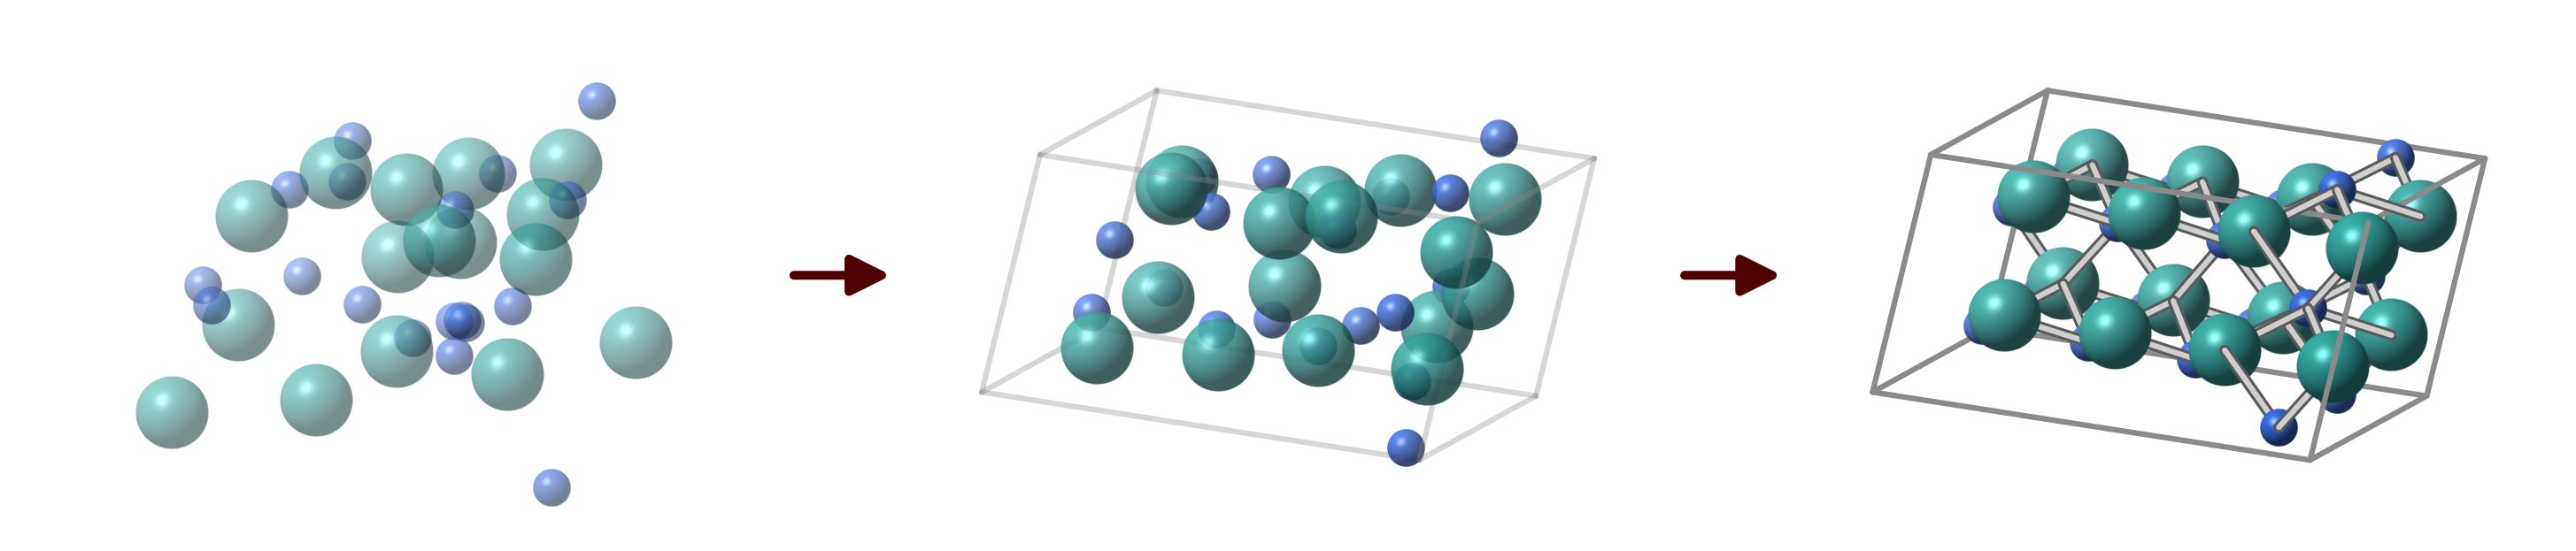
\includegraphics[width=20.6cm]{figs/fig_denoise.png}};

% ---- relax + filter
\node[layer,minimum width=\BW cm,minimum height=2.8cm,anchor=north west]
  (sun) at (\L,21.5) {};
\node[lbl,anchor=west] at ([xshift=0.7cm]sun.west) {Relax + filter};
\node[sub,anchor=east] at ([xshift=-0.7cm]sun.east) {stable, unique, novel};

% ---- the gate
\node[layer,fill=white,draw=AggieMaroon,line width=2.4pt,
      minimum width=\BW cm,minimum height=7.0cm,anchor=north west]
  (gate) at (\L,17.2) {};
\node[lbl,anchor=north west] at ([shift={(0.7,-0.45)}]gate.north west) {Gate};
\node[sub,anchor=north east] at ([shift={(-0.7,-0.58)}]gate.north east)
  {the only change to ungated fine-tuning};
\node[chip] (gp)  at ([yshift=-0.10cm]gate.center) {Gaussian process};
\node[chip,anchor=east] (orb) at ([xshift=-1.25cm]gp.west) {ORB + PCA};
\node[chip,anchor=west] (ei)  at ([xshift=1.25cm]gp.east)  {EI + diversity};
\draw[flow] (orb.east) -- (gp.west);
\draw[flow] (gp.east) -- (ei.west);
\node[note,anchor=south] at ([yshift=0.50cm]gate.south)
  {ranks every survivor; the rest earn no reward};

% ---- oracle
\node[fill=AggieMaroon,minimum width=\BW cm,minimum height=3.8cm,
      anchor=north west,rounded corners=5pt] (orc) at (\L,8.0) {};
\node[anchor=north west,text=white,font=\fontsize{28}{32}\selectfont\bfseries]
  at ([shift={(0.7,-0.50)}]orc.north west) {Property oracle};
\node[anchor=south west,text=PanelGrey,font=\fontsize{22}{26}\selectfont]
  at ([shift={(0.72,0.50)}]orc.south west)
  {learned potential: phonons ($C_p$), equation of state ($K_{\mathrm{VRH}}$)};

% ---- policy update
\node[layer,minimum width=\BW cm,minimum height=2.8cm,anchor=north west]
  (upd) at (\L,2.8) {};
\node[lbl,anchor=west] at ([xshift=0.7cm]upd.west) {Policy update};
\node[sub,anchor=east] at ([xshift=-0.7cm]upd.east) {REINFORCE};

% ---- flow
\draw[flow] (gen.south) -- (sun.north);
\node[note,anchor=west] at ([shift={(0.5,-0.80)}]gen.south) {about 16 candidates per cycle};
\draw[flow] (sun.south) -- (gate.north);
\draw[flow] ([xshift=3.4cm]gate.south) -- ([xshift=3.4cm]orc.north);
\node[notem,anchor=west] at ([shift={(3.95,-1.10)}]gate.south) {top 4 per cycle};
\draw[back] ([xshift=-3.4cm]orc.north) -- ([xshift=-3.4cm]gate.south);
\node[note,anchor=east] at ([shift={(-3.95,-1.10)}]gate.south) {labels train the GP};
\draw[flow] (orc.south) -- (upd.north);
\node[note,anchor=west] at ([shift={(0.5,-0.70)}]orc.south) {rewards};

% ---- next cycle (left) and ungated bypass (right)
\coordinate (lx) at (0.50,0);
\coordinate (rx) at (25.00,0);
\draw[flow] (upd.west) -- (lx |- upd.west) -- (lx |- gen.west) -- (gen.west);
\node[note,rotate=90,anchor=center] at (1.25,15.0) {next cycle};
\draw[bypass] (sun.east) -- (rx |- sun.east) -- (rx |- orc.east) -- (orc.east);
\node[note,rotate=-90,anchor=center] at (24.25,13.1) {ungated: every survivor is evaluated};

\end{tikzpicture}}%
}
